
%(BEGIN_QUESTION)
% Copyright 2011, Tony R. Kuphaldt, released under the Creative Commons Attribution License (v 1.0)
% This means you may do almost anything with this work of mine, so long as you give me proper credit

This water filtration system has a problem.  Examine the faceplate data for all four loop controllers (shown in red text, near each controller) for evidence of the fault:

$$\includegraphics[width=15.5cm]{i00133x01.eps}$$

Identify the likelihood of each specified fault for this system.  Consider each fault one at a time (i.e. no coincidental faults), determining whether or not each fault could independently account for {\it all} measurements and symptoms in this water filtration system.

% No blank lines allowed between lines of an \halign structure!
% I use comments (%) instead, so that TeX doesn't choke.

$$\vbox{\offinterlineskip
\halign{\strut
\vrule \quad\hfil # \ \hfil & 
\vrule \quad\hfil # \ \hfil & 
\vrule \quad\hfil # \ \hfil \vrule \cr
\noalign{\hrule}
%
% First row
{\bf Fault} & {\bf Possible} & {\bf Impossible} \cr
%
\noalign{\hrule}
%
% Another row
Filtering media clogged &  &  \cr
%
\noalign{\hrule}
%
% Another row
FV-44 failed wide open &  &  \cr
%
\noalign{\hrule}
%
% Another row
FV-44 failed fully shut &  &  \cr
%
\noalign{\hrule}
%
% Another row
FV-35 failed wide open &  &  \cr
%
\noalign{\hrule}
%
% Another row
FV-35 failed fully shut &  &  \cr
%
\noalign{\hrule}
%
% Another row
FT-44 failed with high signal &  &  \cr
%
\noalign{\hrule}
%
% Another row
FT-35 failed with high signal &  &  \cr
%
\noalign{\hrule}
%
% Another row
Effluent pump shut off &  &  \cr
%
\noalign{\hrule}
} % End of \halign 
}$$ % End of \vbox

Based on what you see here, is the situation urgent or not?  If you were the operator, what would be your first step in rectifying this situation?

\vskip 20pt \vbox{\hrule \hbox{\strut \vrule{} {\bf Suggestions for Socratic discussion} \vrule} \hrule}

\begin{itemize}
\item{} Which details in this diagram were most helpful for determining the nature and location of the problem?
\end{itemize}

\underbar{file i00133}
%(END_QUESTION)





%(BEGIN_ANSWER)

\noindent
{\bf Partial answer:}


% No blank lines allowed between lines of an \halign structure!
% I use comments (%) instead, so that TeX doesn't choke.

$$\vbox{\offinterlineskip
\halign{\strut
\vrule \quad\hfil # \ \hfil & 
\vrule \quad\hfil # \ \hfil & 
\vrule \quad\hfil # \ \hfil \vrule \cr
\noalign{\hrule}
%
% First row
{\bf Fault} & {\bf Possible} & {\bf Impossible} \cr
%
\noalign{\hrule}
%
% Another row
Filtering media clogged &  &  \cr
%
\noalign{\hrule}
%
% Another row
FV-44 failed wide open &  & $\surd$ \cr
%
\noalign{\hrule}
%
% Another row
FV-44 failed fully shut &  &  \cr
%
\noalign{\hrule}
%
% Another row
FV-35 failed wide open &  &  \cr
%
\noalign{\hrule}
%
% Another row
FV-35 failed fully shut & $\surd$ &  \cr
%
\noalign{\hrule}
%
% Another row
FT-44 failed with high signal &  &  \cr
%
\noalign{\hrule}
%
% Another row
FT-35 failed with high signal &  &  \cr
%
\noalign{\hrule}
%
% Another row
Effluent pump shut off &  &  \cr
%
\noalign{\hrule}
} % End of \halign 
}$$ % End of \vbox

%(END_ANSWER)





%(BEGIN_NOTES)

% No blank lines allowed between lines of an \halign structure!
% I use comments (%) instead, so that TeX doesn't choke.

$$\vbox{\offinterlineskip
\halign{\strut
\vrule \quad\hfil # \ \hfil & 
\vrule \quad\hfil # \ \hfil & 
\vrule \quad\hfil # \ \hfil \vrule \cr
\noalign{\hrule}
%
% First row
{\bf Fault} & {\bf Possible} & {\bf Impossible} \cr
%
\noalign{\hrule}
%
% Another row
Filtering media clogged & $\surd$ &  \cr
%
\noalign{\hrule}
%
% Another row
FV-44 failed wide open &  & $\surd$ \cr
%
\noalign{\hrule}
%
% Another row
FV-44 failed fully shut &  & $\surd$ \cr
%
\noalign{\hrule}
%
% Another row
FV-35 failed wide open &  & $\surd$ \cr
%
\noalign{\hrule}
%
% Another row
FV-35 failed fully shut & $\surd$ &  \cr
%
\noalign{\hrule}
%
% Another row
FT-44 failed with high signal &  & $\surd$ \cr
%
\noalign{\hrule}
%
% Another row
FT-35 failed with high signal &  & $\surd$ \cr
%
\noalign{\hrule}
%
% Another row
Effluent pump shut off &  & $\surd$ \cr
%
\noalign{\hrule}
} % End of \halign 
}$$ % End of \vbox


We can see from the answer that the clearwell controller thinks the clearwell is nearly empty while the influent flow controller and the filter level controller both recognize we have lots of water entering the system.  However, flow controller 35 can't seem to get much water out of the filter even though it's trying hard to open the valve.  Thus, we either have a valve problem (FV-35) or a filter problem.

%INDEX% Basics, control loop troubleshooting
%INDEX% Process: water filter flow/level control

%(END_NOTES)


